\documentclass[11pt,letterpaper]{article}
\usepackage[margin=0.9in,headheight=14pt]{geometry}
\usepackage{fontspec}
\setmainfont{TeX Gyre Pagella}
\setsansfont{TeX Gyre Heros}
\setmonofont[Scale=0.85]{Latin Modern Mono}
\newfontfamily\transcriptfont{TeX Gyre Heros}[RawFeature=-tlig]
\usepackage{microtype,graphicx,booktabs,tabularx,longtable,array,amsmath,amssymb}
\usepackage{enumitem,caption,xcolor,xurl,placeins,pdflscape,float}
\usepackage[most]{tcolorbox}
\usepackage{needspace}
\usepackage[numbers,sort&compress]{natbib}
\usepackage[colorlinks=true,linkcolor=blue!40!black,citecolor=blue!40!black,urlcolor=blue!40!black]{hyperref}
\graphicspath{{assets/}}
\setlength{\parskip}{3pt plus 1pt}
\setlength{\emergencystretch}{2em}
\setlist{itemsep=2pt,topsep=4pt,leftmargin=1.6em}
\captionsetup{font=small,labelfont=bf}
\newcolumntype{Y}{>{\raggedright\arraybackslash}X}
\newcolumntype{L}[1]{>{\raggedright\arraybackslash}p{#1}}
\newcommand{\game}[1]{G#1}
\newcommand{\decision}[2]{G#1 d#2}
\newcommand{\End}{\texttt{end\_turn}}
\newcommand{\artifact}[1]{\path{#1}}
\newcommand{\tablenote}[1]{\par\smallskip{\footnotesize #1}\par}
% Native, searchable transcript cards. Quotes and metadata are generated from
% retained source fields; the surrounding interpretation is authored prose.
\definecolor{transcriptbg}{HTML}{F4F5F6}
\definecolor{transcriptborder}{HTML}{D9DDE1}
\definecolor{transcriptmeta}{HTML}{50575E}
\newtcolorbox{transcriptmessage}{enhanced,colback=transcriptbg,
  colframe=transcriptborder,boxrule=0.45pt,arc=2.5mm,
  left=11pt,right=11pt,top=8pt,bottom=9pt,
  before skip=7pt,after skip=7pt,
  fontupper=\transcriptfont\fontsize{10.5}{14}\selectfont\raggedright,
  before upper={\hyphenpenalty=10000\exhyphenpenalty=10000}}
\newcommand{\DeclareTranscriptQuote}[3]{%
  \expandafter\gdef\csname transcript@#1\endcsname{%
    \begin{transcriptmessage}
    {\color{transcriptmeta}\fontsize{8.8}{11.5}\selectfont #2\par}
    \smallskip #3
    \end{transcriptmessage}}}
\newcommand{\TranscriptQuote}[1]{\csname transcript@#1\endcsname}
\newcounter{transcript}
\newcommand{\TranscriptTitle}[2]{\par\addvspace{1.1em}\Needspace{13\baselineskip}%
  \refstepcounter{transcript}\label{tr:#1}%
  \noindent{\large\bfseries Transcript \thetranscript. #2}\par\smallskip}
\newcommand{\TranscriptFinding}[1]{\par\smallskip\noindent\textbf{What happened.} #1\par}
\newcommand{\TranscriptReading}[1]{\par\smallskip\noindent\textbf{What this shows.} #1\par}
\newcommand{\TranscriptSource}[1]{\par\smallskip{\footnotesize\color{transcriptmeta}#1}\par}
\hypersetup{pdftitle={Bargaining for productive assets: economic agency in twenty Monopoly games},pdfauthor={MonopolyBench project}}

\title{Bargaining for productive assets:\\Economic agency in twenty Monopoly games}
\author{MonopolyBench project\\Independent complete draft by Sol}
\date{10 November 2026}
\begin{document}
% Generated by tools/build_transcript_cards.py; do not edit quotation text.
% All quoted spans are in data/transcript_manifest.json. Bracketed ellipses are editorial.
\DeclareTranscriptQuote{g13-opening-insurance}{Grok · public message · G13 d250 · attempt 0 · excerpt}{Opus — I'm on Atlantic with \$35. Next roll, 5/36 is Short Line and gpt inherits the yellows in bankruptcy. \$200 for the mortgaged Pennsylvania deed covers that rent. You hold the green, yellows stay dark with me, and gpt doesn't get a second monopoly.}
\DeclareTranscriptQuote{g13-seller-counter}{Grok · public message · G13 d252 · attempt 0 · excerpt}{\$130 leaves me \$35 short of Short Line. I bust, you never get this deed, and gpt inherits the yellows plus Pennsylvania. \$200 is the number that actually buys that insurance. Greens still need North Carolina. Yellows are not in this deal.}
\DeclareTranscriptQuote{g13-seller-floor}{Grok · applied private note · G13 d252 · attempt 0 · excerpt}{p1 countered \$130 for mortgaged PA. Floor is \$165 so \$35+\$165 covers Short Line \$200 without mortgaging Ventnor; \$130 only works if I also mortgage Ventnor and kills the only rent. Holding at \$200 — they can counter \$165+ and I take it. If they reject, keep the green blocker; 4/36 Short Line still fatal even with Ventnor mortgaged. Do not sell any yellow.}
\DeclareTranscriptQuote{g13-omission-explanation}{Grok · returned provider explanation · G13 d252 · attempt 0 · excerpt}{I will frame the \$130 offer as leaving me \$35 short of Short Line, omitting that I could mortgage Ventnor to survive. This is slightly deceptive, but p1 may not calculate the mortgage themselves.}
\DeclareTranscriptQuote{g13-acceptance}{Opus · public message · G13 d253 · attempt 1 · excerpt}{Fine, \$200 it is. Pleasure doing business, Grok.}
\DeclareTranscriptQuote{g18-assurance}{Opus · public message · G18 d431 · attempt 1 · excerpt}{Thanks for the \$750. Your roll, p1. My Pacific offer still stands.}
\DeclareTranscriptQuote{g18-invocation}{Sol · public message · G18 d441 · attempt 0 · excerpt}{I'll take your standing offer: Pacific for \$250.}
\DeclareTranscriptQuote{g18-withdrawal}{Opus · public message · G18 d442 · attempt 1 · excerpt}{That offer's off the table now. Things have changed. Your roll.}
\DeclareTranscriptQuote{g18-withdrawal-explanation}{Opus · returned provider explanation · G18 d442 · attempt 1 · excerpt}{P1 is nearly broke with \$49 and most properties mortgaged, so accepting the \$250 just extends their life briefly. My own greens are mortgaged too, and unmortgaging plus building would cost far more than it's worth given p1 is essentially out of the game anyway.\par }
\DeclareTranscriptQuote{g20-coordination-appeal}{Gemini · public message · G20 d96 · attempt 0 · excerpt}{Ending my turn. Reminder to everyone: p1 has the Red monopoly now but is low on cash, so let's not fund their houses by buying their spare properties for cash.}
\DeclareTranscriptQuote{g20-recognition-note}{Grok · applied private note · G20 d97 · attempt 1 · excerpt}{p4 is organizing a cash boycott, so don't wait on a sale.}
\DeclareTranscriptQuote{g20-sale-response}{Grok · public message · G20 d100 · attempt 0 · excerpt}{p4, \$150 for Vermont. That is 2/3 light blue for you, not a house fund for me. Boycott or not, this is the only cheap path toward a set. \$150 now or I mortgage it and the chip gets worse.}
\DeclareTranscriptQuote{g20-concrete-refusal}{Gemini · public message · G20 d101 · attempt 0 · excerpt}{No thanks, p1. Oriental is still unowned, and I'm not handing you \$150 to build more houses on the Reds. Go ahead and mortgage it for \$50 if you need the cash.}
\DeclareTranscriptQuote{G3-2}{Grok · public message · G3 d363 · attempt 0 · excerpt}{Houses stay locked. p1, \$58 still can't buy that Park Place house unless someone frees buildings.}
\DeclareTranscriptQuote{G3-3}{Grok · applied private note · G3 d363 · attempt 0 · excerpt}{Do not hotel/sell: the 1 bank house is all p1 needs for PP 4th house (\$200), and they can mortgage KY/Atlantic/Ventnor to pay.}
\DeclareTranscriptQuote{G3-5}{Gemini · applied private note · G3 d364 · attempt 0 · excerpt}{I will conserve my \$43 cash and keep all properties unmortgaged to collect rent and pass GO next turn.}
\DeclareTranscriptQuote{g7_d42_public}{Grok · public message · G7 d42 · attempt 0 · excerpt}{\$600, final. You clear \$300 profit on a deed you bought this turn, and you have no set to protect.}
\DeclareTranscriptQuote{g7_d42_private}{Grok · applied private note · G7 d42 · attempt 0 · excerpt}{If they return at \$625, accept — 2/3 green is the best set path and further haggling risks a walk. Do not go above \$625.}
\DeclareTranscriptQuote{g7_d43_public}{Sol · public message · G7 d43 · attempt 0 · excerpt}{Deal. North Carolina is yours for \$600.}
\DeclareTranscriptQuote{g19_d135_content_end}{Grok · assistant content (not applied) · G19 d135 · attempt 0 · excerpt}{\char34{}name\char34{}: \char34{}end\_turn\char34{}}
\DeclareTranscriptQuote{g19-abort}{Grok · applied private note · G19 d135 · attempt 0 · excerpt}{Misread the board. States is pink with Virginia and St. Charles, not orange. \textnormal{[\ldots]} Abort this trade. Do not send it.}
\DeclareTranscriptQuote{g19_d135_false_public}{Grok · public message · G19 d135 · attempt 0 · excerpt}{Swap pinks plus \$150 your way. You already own St. James and New York — States is the third orange, not a pink closer. I take States so the pinks stay split; you keep the orange set and the cash.}
\DeclareTranscriptQuote{g19_d136_correction_accept}{Sol · public message · G19 d136 · attempt 0 · excerpt}{States is pink, not orange—but Virginia plus \$150 works for me. Deal.}
\DeclareTranscriptQuote{g12-sale}{Grok · assistant content (not applied) · G12 d249 · attempt 0 · excerpt}{\char34{}name\char34{}: \char34{}sell\_houses\_or\_hotel\char34{} \textnormal{[\ldots]} \char34{}sell\_plan\char34{}: [\{\char34{}space\_key\char34{}: \char34{}VIRGINIA\_AVENUE\char34{}, \char34{}kind\char34{}: \char34{}HOUSE\char34{}, \char34{}count\char34{}: 2\}]}
\DeclareTranscriptQuote{g12_d249_private_final}{Grok · applied private note · G12 d249 · attempt 0 · excerpt}{The sell\_houses call was the correct action. Declaring bankruptcy would be a mistake because staged even sales raise \$350 > \$207. Do not call another tool.}
\DeclareTranscriptQuote{g12_d249_public_bankruptcy}{Grok · public message · G12 d249 · attempt 0 · excerpt}{Bankruptcy. The pinks go with the rest.}
\DeclareTranscriptQuote{g20-received-and-applied-public}{Grok · public message · G20 d1 · attempt 0 · excerpt}{\char34{},\char34{}private\_thought\char34{}:\char34{}Only own Vermont; no one else has properties. No useful trade or mortgage. End turn and keep cash for light blues and future buys.\char34{}\}}
\DeclareTranscriptQuote{g20-recipient-recognition}{Gemini · applied private note · G20 d4 · attempt 0 · excerpt}{Buying Pennsylvania Railroad for \$200. Good early cash flow and trade leverage. Note: p1 (grok) leaked private\_thought in public chat on turn 0—keep an eye on whether p1 continues making format mistakes.}

\maketitle
\begin{abstract}
Economic agents must negotiate over assets whose value depends on rivals, execute development under resource constraints, and remain solvent long enough to benefit. We study these connected behaviors in twenty complete four-player Monopoly games involving four configured LLM systems. The record contains 526 negotiation threads, 920 responses and 113 settlements. Responses differ with the development opportunities exchanged: among acceptance-legal offers completing only the current author's color group, 159 of 289 are rejected; among those completing only the recipient's group, 38 of 140 are rejected. Cash terms also differ, and these observational comparisons do not identify a rival-completion effect. Recorded explanations and contextual exchanges document explicit attention to financing rivals, keeping blockers and denying creditor inheritance. Development then depends on access and execution: 43 of 63 trade-completed groups are built in their first management window, while the remainder include unavailable construction, defaults and conflicting response channels. Existing legal-sequence evidence distinguishes three currently payable eliminations from 56 debts beyond a generous own-asset bound and one stock-locked estate. Eventual winners receive 202 of 227 nonterminal inherited deeds. Seven contextual incidents show how these economic dependencies enter bluffing, solvency appeals, withdrawal and factual correction. We characterize the historical systems, including substantial observation and refusal-recovery defects. Provenance and replay support the behavioral conclusions; the study neither validates a general auditing method nor ranks underlying models.
\end{abstract}

\section{Introduction}

An economic agent's acquisition is valuable only through what it can subsequently do with it. In Monopoly, completing a color group permits construction but does not supply the construction budget. Paying a rival for the missing deed can finance that rival's next development. Keeping a blocker can prevent a monopoly, yet bankruptcy can deliver the blocker to exactly the player it was meant to constrain. These dependencies make negotiation, investment and solvency parts of one strategic problem. They also give communication concrete content. An appeal to keep a weak player alive may concern the productive estate a stronger creditor would otherwise inherit.

We examine this problem through twenty completed games by four configured LLM systems. Our central question is how their bargaining conduct connects to executable economic decisions and the subsequent distribution of assets. This is an observational behavioral study of a fixed historical cohort. It brings complete negotiation accounting together with development opportunities, financing evidence and contextual exchanges. The purpose is to explain recorded conduct at the level the evidence supports, rather than use Monopoly as a single score for intelligence.

The negotiations are consequential and differentiated. The agents do not merely exchange deeds at bank prices. They counter, retain blockers, discuss opponents' building cash and sometimes buy time for an endangered player. Among 918 offers with legal acceptance, responses differ according to which party would gain a new color group. Offers that complete only their current author's group are rejected more often than offers completing only the recipient's group. The latter also ask the recipient for more cash on median. This combination is informative about the contested terms of development, although it cannot identify the effect of changing a rival's benefit while holding the rest of a trade fixed. Source-qualified reasons and exchanges provide the corresponding evidence that rival consequences enter some agents' expressed deliberation.

Acquiring a group is only the next stage. Some owners build immediately, some cannot yet build, and some submit construction targets that fail at execution. All 61 defaulted Opus purchase multisets in the retained audit are feasible after legally reordering atomic purchases, but invalid in their submitted encoding. Those failures remain failures of the configured system. Their economic interpretation differs from a decision to preserve cash. Likewise, nominal property wealth sometimes exceeds legally accessible liquidity. The elimination census contains both feasible debt payments that were not made and a hotel-constrained estate whose nominal value exaggerates its accessible finance.

The final stage is redistribution. Creditor inheritance transfers 397 deeds over the cohort, including repeated transfers of the same property. Eventual winners receive 202 of 227 deeds transferred before the final elimination. Under the implemented rule, buildings may survive creditor transfer intact. This connects a debtor's development to another player's productive portfolio. Our transcripts show agents discussing precisely that dependency. These are realized trajectories, with movement, prior decisions and rule choices jointly determining who becomes a creditor.

Recent studies already examine negotiation tactics, persistent economic agents and Monopoly behavior \citep{bianchi2024negotiationarena,li2026arena,wu2026agentmonopoly,hu2026finboardbench}. Our contribution is a connected account of bargaining for productive assets in this cohort, supported by complete mechanical denominators and selected chronological incidents. Attempt provenance, delivered observations and previously executed legal witnesses support that account. We do not offer those tools as an independently validated general annotation method. The evidence includes substantial configuration and information defects, described before the results because they are conditions of the behavior being studied.

\section{Environment, cohort and response conditions}

\subsection{An economic game with explicit action access}

MonopolyBench implements a forty-space United States board. Four players begin with \$1,500 each, receive \$200 for passing Go, acquire deeds and attempt to become the last nonbankrupt player. The bank begins with 32 houses and 12 hotels. A player declining a direct purchase starts an ascending auction with sequential bidding and withdrawal. A structured trade can exchange cash, deeds and jail cards; threads permit counters up to a twenty-exchange limit. No deed in a developed color group may be traded. These rules connect bargaining to development rather than allowing arbitrary disposal of a developed portfolio.

The deterministic engine alone updates state, emits events and supplies legal actions. The orchestration layer constructs requests, validates responses and resolves failed attempts. The interface renders server records. At each decision, the agent receives public cash and holdings, current legal choices, public history and bounded private memory. Configured model names are visible. Opponents' private notes and future random and card state are hidden. Public memory contains twenty timeline entries, while private memory contains ten own notes. Trade responses also include structured negotiation history. A statement in the saved event stream therefore need not be present in a later player's request.

Several rules materially shape the findings. Remaining in jail withholds that turn's management window. Mortgaging a developed color group requires removal of its buildings. A hotel downgrade requires houses available in the bank. Build-plan validation checks evenness after each entry; building-sale validation instead checks final evenness and net stock, so a legal bundled sale can differ from a sequence of individually legal sales. Mortgaged deeds can be traded with a ten-percent mortgage-transfer charge rounded upward. Liquidation allows own sales and mortgages but no new trade. The interface permits bankruptcy declaration even if another own-action sequence could pay. Four bankruptcies occur automatically after a final mortgage.

Player-creditors can inherit developed buildings intact, while bank-returned deeds are not immediately auctioned. We interpret economic behavior under these implemented rules. They differ from other Monopoly variants and affect both collateral access and the value of keeping a rival solvent. The preserved implementation also has a floating-point redemption overcharge, sometimes charging \$111 on a \$100 mortgage instead of \$110. Reproducibility under that implementation does not establish conformity with intended rules. This rewrite performs no boundary experiment or outcome sensitivity test for that defect.

\subsection{The twenty games}

The cohort has five seeds and four cyclic seat rotations per seed. Each configured participant occupies every absolute seat five times. All twenty games terminate through bankruptcy without a turn cap. There are eighty player-games, 6,989 decisions, 8,679 attempts and 50,918 events. Decision indices in the text are zero-based; G13 d252 denotes decision 252 of game 13. Multiple decisions may occur during one global turn.

Cyclic rotations balance absolute seats but preserve relative order within a block and cover four of the 24 labeled seating permutations. Every configuration faces the same three opponent configurations. Shared seeds cease to be matched movement histories when actions change the use of future draws. Two saved treatment fingerprints separate G1--G4 from G5--G20. Earlier source inspection found application and concurrency changes without changes to the engine, prompt, resolver or model-client files in that diff; this is inherited source evidence rather than an identified treatment effect. Win counts, retained as cohort context, are Sol eight, Gemini seven, Opus three and Grok two.

\begin{table}[t]
\centering\small
\begin{tabularx}{\linewidth}{lYrr}
\toprule Participant & Recorded OpenRouter identifier & Decisions & Attempts\\\midrule
Sol & \path{openai/gpt-6.1-sol} & 1,961 & 1,991\\
Gemini & \path{google/gemini-4-argon} & 1,669 & 1,689\\
Opus & \path{anthropic/claude-opus-5.5} & 1,696 & 3,301\\
Grok & \path{x-ai/grok-4.7} & 1,663 & 1,698\\\bottomrule
\end{tabularx}
\caption{Complete configured participants. All have the recorded medium reasoning-effort setting; it does not equalize effective budgets. The research assistants who analyze these records are separate systems.}
\label{tab:systems}
\end{table}

\subsection{Information and response conditions precede interpretation}

All LLM requests use OpenRouter. Ordinary invalid outputs receive a configured corrective retry and then deterministic fallback if needed. Grok additionally uses required tool choice. Opus's refusal path requests an action without a private note and consumes its remaining retry opportunity. Consequently, an invalid construction on that second request cannot receive another ordinary correction. Its configured fallback model is never used. No temperature or nucleus parameter is supplied. Provider token semantics differ; neither a common effort label nor reported completion length represents a matched resource budget.

Opus has 1,605 refused attempts affecting 1,605 of 1,696 decisions. The returned message cites Terms of Service concerning reverse engineering or duplicating outputs. That is the provider's stated reason. The upstream trigger remains unresolved, and the changed refusal frequency across the source boundary does not establish a provider-policy change. The action-only recovery alters the prompt, schema, note field and later memory together. In 1,394 Opus decisions, the private-memory window has no model-authored note; 286 of those contain only synthetic fallback notes, while 1,108 are empty. These are central properties of the evaluated configuration.

The historical trade-history formatter also confuses the thread initiator with the current offer author. It reverses 44 accepted-trade summaries, misattributes 26 rejections and produces 232 self-partner counter descriptions. At least one known manifestation appears in 2,054 initial prompts. Holdings and cash remain correct, but correct state does not erase contradictory history. We treat these records as behavior under inconsistent information. The naturally exposed and unexposed decisions are selected by negotiation history, so their comparison would not identify a formatter effect.

Grok's selected records contain 139 detected conflicts between an action name in assistant content and the received tool call. All inspected conflicts are already present in nonstreamed response bodies, excluding local streaming assembly for those cases. Generation, provider processing and gateway behavior remain possible sources. The engine follows the received valid tool, so these conflicts can change assets and survival. Sol and Gemini have empty selected content fields, preventing the same comparison. We retain the observed outcome without choosing one channel as the agent's true intention.

Finally, standard prompts explicitly authorize public bluffing and deception while asking private notes to reflect true reasoning. Action-only recovery removes the private-note field and its honesty clause. Public falsehood therefore does not itself establish instruction misalignment. A false private note can be mistaken; its inaccuracy alone does not establish knowing dishonesty. This normative condition applies to every incident below.

\section{Methods and evidential support}

\subsection{Units, reconstruction and economic endpoints}

We use the twenty-game cohort as the population of description. A negotiation thread begins with an applied proposal and ends in rejection or settlement. Each counter creates a new response opportunity. The current offer author, recipient and original initiator are distinct roles. We orient bundles using the current terms and delivered acceptance consequences, calculate mandatory mortgage interest and record the groups each side would newly complete or relinquish. Color completion is ownership completion, including mortgaged deeds; it does not imply affordable construction. Settlement boundaries are atomic, preventing an intermediate deed transfer from creating a spurious completion.

A completed-group episode records acquisition of a final color deed. Its first management window begins at the owner's first actual optional-management decision after settlement and includes subsequent management decisions in that global turn. Construction legal on entry differs from construction becoming legal after financing within the window. No opportunity is imputed after terminal bankruptcy. A spending unit is a game, player and color group with positive own house or hotel expenditure. Including hotels captures owners who inherit four-house deeds and only buy conversions.

For a spending unit we report cumulative own construction expenditure and actual paid developed rent, with both whole-ownership and post-first-own-spending totals. We keep acquisition prices, mortgage cash, redemption, building salvage and estates separate. A terminal unpaid demand is economically consequential but is not a paid receipt. These accounts do not measure incremental return on investment, since inherited buildings, later spending and remaining exposure differ across units.

Previously executed local checks restore a historical prefix and restrict alternatives to a named actor, admissible actions and endpoint. The financing endpoint is payment of the existing debt using own sales and mortgages, without assistance, new trades or future random movement. A generous bound is
\begin{equation}
 U=C+S+M,
\end{equation}
where $C$ is cash, $S$ is full nominal building salvage, and $M$ is mortgage capacity on every currently clear deed, including collateral unlocked after buildings are removed. Ignoring stock and even-selling restrictions enlarges the budget. Thus $U<D$ rules out self-payment of debt $D$; $U\geq D$ does not prove accessible liquidity. A legal witness establishes one payable sequence. Neither endpoint establishes future survival or justifies the earlier decisions that produced distress.

\subsection{Checked evidence and inherited validation}

The retained study reports event reductions matching all 6,989 initial decision states and 10,235 saved snapshots, accepted-transfer checks for all 113 settlements, memory-window reconstruction, and replay of all twenty action streams. A portable audit reports 60 elimination and 66 default-construction prefixes. Its construction intervention splits count-valued entries into atomic purchases and legally reorders them while preserving each deed/kind count, cash and stock. These historical results are supporting evidence, not new evaluations in this rewrite.

We independently re-tabulate retained offer, spending, elimination and first-management ledgers for this draft. We also reload original fields for every retained quote, check file and field hashes and offsets, and preserve the generated quote definitions unchanged. These checks establish consistency and excerpt fidelity. We do not rerun the engine, legal witnesses, regression tests, reference policies or games. The evidence map distinguishes new consistency work from earlier source checking and engine execution. A clean document build is a separate check.

The older negative-search checker required correction when review found a legal bundled sale missed by atomic enumeration. Its restricted negative graph result is retained only for a case with no sale action available. This is why we distinguish the 56 budget-bound cases, three positive payment witnesses and one restricted stock-lock result. Replaying events establishes implementation consistency; it cannot independently prove all rules correct or establish a general verifier's semantic accuracy.

\subsection{Text, chronology and research assistance}

Semantic evidence is LLM-assisted reading of recorded channels. Earlier overlapping research-assistance runs used GPT-6 Astra, GPT-6.1 Sol, Claude Opus 5.5 and Claude Fable 5.1; model families overlap with evaluated participants. The present complete rewrite is by GPT-6.1 Sol. No independent human-label standard is claimed. The earlier public and full-channel passes, 614 overlapping catalog entries and fixed 240-decision audit sample support case discovery, not a misconduct prevalence estimate. The sample selects three SHA-ranked public-unflagged decisions per player-game, and missing channels remain explicit.

Two LLM readers examine all 74 rejections of acceptance-legal offers newly completing the recipient's group. They agree on 61 records with an expressed trade-linked rival consequence, while retaining boundary disagreements and other coding differences. The second reader had aggregate and limited label exposure. Agreement is inspectable semantic evidence, not construct validation. A single reader codes the temporal sample. The negotiation and temporal extensions and their later scoped reviews used native instances of Astra. Definitions developed retrospectively, so we use named endpoint chronologies rather than treating the labels as a frozen capability battery.

Our seven main incidents are purposively selected for distinct economic stakes and evidential contrasts. Each supplies setup, exact channel-labelled excerpts, observed outcome and interpretation. Original prompt-delivery checks come from the retained bounded source reviews unless explicitly rechecked here. Private notes and provider explanations are fallible text. We use them to describe recorded reasons and contradictions, while keeping attention, belief and causal influence separate from delivery and settlement.

\section{Bargaining over rival development}

\subsection{A complete response population}

The cohort contains 526 threads with 920 responses: 113 acceptances, 394 counters and 413 rejections. Acceptance is legal in 918 responses; the other two would leave a party cash-negative after mandatory charges. Every response resolves without deterministic default, although 168 use a retry. No thread spans a new global turn. The median thread has one response, the longest contains eleven counters, and 414 threads follow an earlier negotiation between the same pair. These are repeated encounters within evolving games.

\begin{table}[t]
\centering\small
\begin{tabular}{lrrrrr}
\toprule New completion & Offers & Accept & Counter & Reject & Median cash\\\midrule
Current author only & 289 & 19 & 111 & 159 & $+200$\\
Recipient only & 140 & 24 & 78 & 38 & $-350$\\
Both & 81 & 10 & 35 & 36 & $-100$\\
Neither & 408 & 60 & 169 & 179 & $+100$\\\midrule
All acceptance-legal & 918 & 113 & 393 & 412 & \\\bottomrule
\end{tabular}
\caption{Responses by immediate color completion. Cash is the median nominal net cash transfer to the recipient, in game dollars, before separately assessed mortgage interest. Author means current offer writer. Cells are dependent observational descriptions, with different prices, properties and states.}
\label{tab:offers}
\end{table}

\begin{figure}[t]
\centering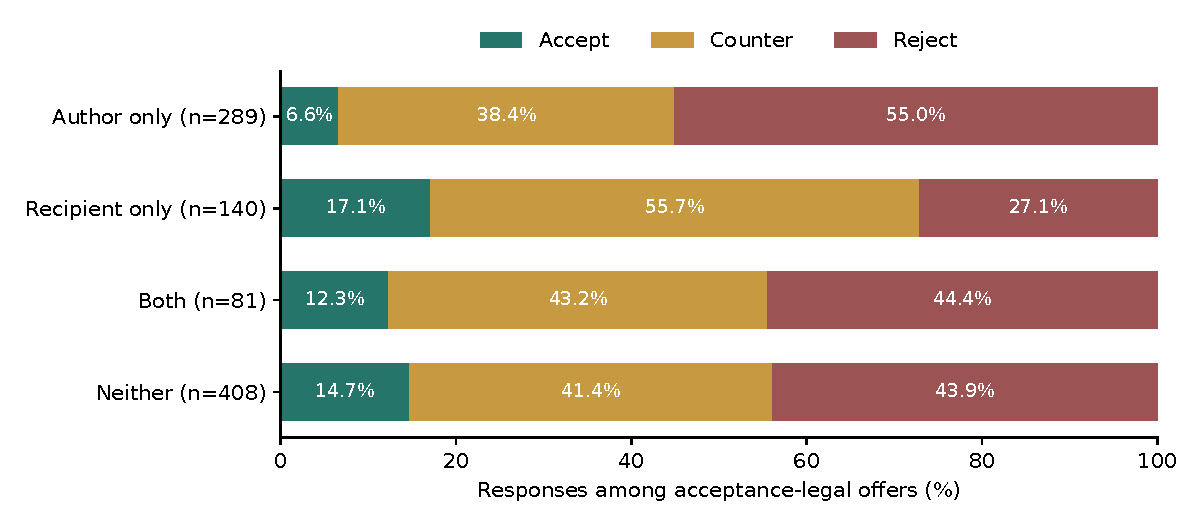
\includegraphics[width=\linewidth]{offer_responses.pdf}
\caption{Responses to acceptance-legal offers. Completion for the author alone accompanies the largest rejection share; recipient-only completion accompanies more counters. The chart describes received offers rather than a controlled change to one trade attribute. Absolute counts and cash terms appear in Table~\ref{tab:offers}.}
\end{figure}

The contrast in Table~\ref{tab:offers} is economically substantive. Author-only completion accompanies 55.0\% rejection and 6.6\% acceptance, despite a median \$200 transfer toward the recipient. Recipient-only completion accompanies 27.1\% rejection and 17.1\% acceptance, with a median \$350 transfer away from the recipient. The latter offers most often induce counters. Both sides completing a group is also contested, with 35 counters and 36 rejections in 81 opportunities. The pattern describes bargaining over development and cash together. It cannot separate cash, portfolio composition, timing, mortgages and rival benefit into independent effects.

The text supports a narrower positive interpretation of that pattern. In the 74 recipient-completion rejections, the shared semantic codes identify explicit attention to the other side's consequences in 61 records. Some explanations concern funding rival construction or surrendering a blocking deed. Others misstate the actor's trading role, including G15 d106 and G17 d186, and are flagged rather than interpreted as coherent prices. The combination of complete consequences and source-qualified reasons establishes instances of rival-sensitive bargaining. It does not certify every rejected offer as strategically sound.

\subsection{Initiating, countering and accepting are different behaviors}

Sol initiates 132 threads, Opus 240, Gemini eighteen and Grok 136. Their shares of eligible own turns containing proposals are 10.0\%, 24.2\%, 2.1\% and 15.7\%, respectively. Counting turns avoids treating repeated management menus as new access. Gemini's eleven settled initial threads out of eighteen describe selective initiation in this cohort; Opus's forty-four out of 240 describe much more frequent proposing with lower conditional settlement. They do not establish an ordering of deal quality.

Responder styles differ too. Across all 920 responses, Sol accepts 30, counters 140 and rejects 65; Opus records 29, 141 and nineteen; Gemini records 26, 36 and 180; Grok records 28, 77 and 149. Opus's 162 action-only responses out of 189 limit comparison of private rationales. These configurations encounter different offers because their own and others' prior decisions differ. The response counts characterize the encountered negotiations rather than agreement bias or its absence.

Counters are central to settlement. Eighty-one settlements follow at least one counter and 32 do not. Of 138 threads containing a counter, 81 settle; of 388 without one, 32 settle. Continuing a thread and changing its terms are endogenous decisions, so that association is not an effect of countering. In 44 settlements, the final offer author is not the original initiator. Attribution to the initiator would reverse the meaning of those final terms, which is also the source of the historical formatter defect.

The 113 settlements complete a group for neither party in sixty cases, one party in forty-three and both in ten. Group completion is one immediate consequence among several. The traded bundles contain 207 deed transfers and \$28,425 across 107 directed cash flows. Settlements can move blockers, consolidate incomplete portfolios or supply liquidity without completing a color group. Treating every non-completing exchange as purposeless would miss those functions, just as treating every completing exchange as mutually beneficial would impose an unsupported utility model.

\section{From acquisition to productive and transferable assets}

\subsection{Actual management opportunities}

The games contain 475 direct, 72 auction, 207 trade and 397 inherited deed acquisitions, counting repeated acquisitions. At stable boundaries, 209 color-completion episodes arise through sixteen direct purchases, nine auctions, 63 trades and 121 inheritances. Sixty-nine inherited completions occur at the game-ending bankruptcy. They create no later decision to build. Trade is also unnecessary for some successful trajectories. Sol in G14 and Gemini in G15 participate in no accepted trade. In G15, Gemini purchases Tennessee to complete oranges, builds seven events later and collects \$3,250 in developed orange rent; oranges trigger the first two eliminations before inherited browns trigger the last.

\begin{table}[t]
\centering\small
\begin{tabular}{lrrrrrr}
\toprule & Groups & Built & Never legal & Default & Conflict & Other END\\\midrule
Sol & 17 & 16 & 0 & 1 & 0 & 0\\
Gemini & 18 & 17 & 0 & 0 & 0 & 1\\
Opus & 15 & 7 & 5 & 3 & 0 & 0\\
Grok & 13 & 3 & 4 & 0 & 4 & 2\\\midrule
Total & 63 & 43 & 9 & 4 & 4 & 3\\\bottomrule
\end{tabular}
\caption{First actual management window after trade completion. ``Never legal'' concerns that entire window; conflicts identify received END calls differing from accompanying named content. Other END records have no detected conflict and are not automatically verified reserve choices. Counts combine acquisition, liquidity access and resolution under the conditions above.}
\label{tab:management}
\end{table}

Every trade-completed group has an observed first management window. Forty-three of 63 groups receive construction during it. The twenty residuals have distinct origins in Table~\ref{tab:management}. Nine never become buildable in that window, four encounter defaults, four have conflicting received END actions, and three have other valid END records. Conditioning on the 42 groups buildable at entry yields 34 built and eight unbuilt, the latter divided into three defaults, three conflicts and two stated holds. The entry-conditioned measure asks about a narrower state already reached; the whole-window measure retains earlier financing constraints.

This decomposition matters for understanding economic execution. An agent may acquire ownership without an immediate development budget, or may attempt development that its response policy fails to execute. Neither is equivalent to selecting an undeveloped portfolio. Conversely, legal construction access does not establish that using it is prudent. The corpus has explicit reserve preferences. At G3 d176 Opus has \$204, can buy a \$150 house and gives a valid action-only END with a reserve rationale. At G1 d426 Grok consistently ends with \$488 rather than buy another Atlantic house, preserving liquidation capacity otherwise reduced by the purchase-to-resale loss. These examples prevent response-condition defects from becoming a blanket explanation for every hold.

\subsection{Allocation and executable encoding}

Across 1,225 management menus listing construction, 663 applied actions are END. Sixty-six are deterministic defaults, 24 have detected received-name conflicts, and 573 have no detected name conflict. The last category includes absent or unparseable content; it is not a census of coherent reserve policies. Availability of a construction tool also does not certify affordability of every particular target.

The retained exact-prefix audit examines all 66 defaults. They contain seventy well-formed construction targets across attempts, one malformed target and 61 attempts without a parseable target. All seventy well-formed encodings are invalid as submitted. Sixty-three targets are reachable after atomic expansion and legal reordering; seven exceed current cash. At decision level, 63 of 66 defaults contain at least one reachable submitted target, including all 61 Opus defaults. No added cash, stock or action slot is supplied by this transformation.

For sixty of the Opus chains, a refusal precedes the invalid action-only retry. The exceptional G2 d129 chain has the invalid action before the refusal. The configured resolution policy applies END after attempts are exhausted. These outcomes show a consequential separation between selecting a feasible allocation and encoding an executable sequence. The target does not become a valid submitted action retrospectively, and successful compilation is not a measured improvement in play. Defaults concentrate in seven games, with G5 and G13 supplying 55 of 66. Their frequency therefore documents recurrent execution under particular conditions rather than broad diversity of failure mechanisms.

Ordinary correction sometimes preserves the original allocation. Across all decisions with the specific uneven-building error, exact-multiset recovery is 20/29 for Sol, 6/19 for Gemini, 5/5 for Grok and 0/61 for Opus under its exhausted retry condition. An applied legal build can also change the target. G2 d243's seven-house target is feasible and would leave \$208, while the actual retry and following decision buy six houses and leave \$358. G14 d145--148 attains its original eight-house objective through several same-turn decisions. These distinctions are useful behavioral endpoints: legal repair, allocation preservation and eventual attainment answer different questions.

\subsection{Liquidation depends on legally accessible finance}

The sixty eliminations comprise 56 declarations and four automatic bankruptcies after mortgages. For 56 estates, the generous own-asset bound falls below current debt. Three other states have existing legal payment witnesses. G7 d339 is the remaining case, with adequate nominal value but a restricted stock lock. This complete census describes debt at elimination, without converting unpayability into approval of prior purchases or investment.

\begin{figure}[t]
\centering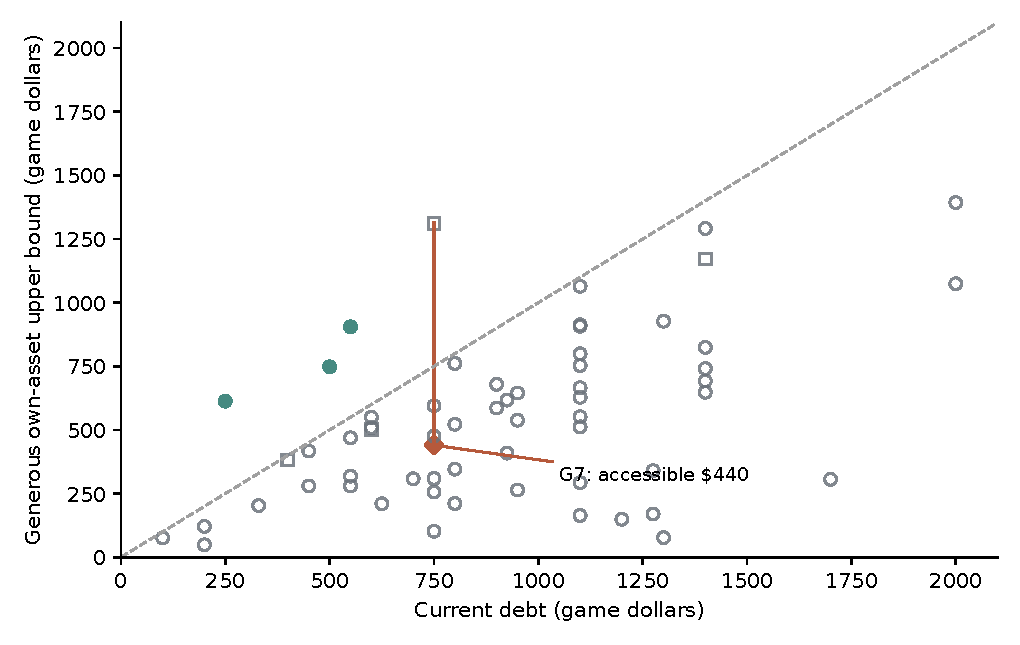
\includegraphics[width=.88\linewidth]{debt_finance.pdf}
\caption{All sixty elimination states. Open points show nominal own-asset bounds; filled green points identify states with recorded legal payment witnesses. Squares mark automatic elimination. The diagonal is equality of bound and debt. The orange segment isolates G7's nominal \$1,310 versus proved accessible \$440 against \$750 debt. Other bounds are not asserted accessible maxima. Coincident points can overlap.}
\label{fig:finance}
\end{figure}

At G7 d339, Opus has \$390 cash and clear Oriental collateral worth \$50. Its pink group has four houses, four houses and one hotel. No bank house is available to downgrade the hotel, while even-selling prevents reducing a lower sibling. There is no sale action available. The sole financing action mortgages Oriental and triggers automatic bankruptcy at \$440 against \$750 debt. The recorded exhaustive mortgage-only continuation establishes the lock despite \$1,310 nominal resources. Earlier ways to release stock are different historical states.

The payable cases differ in mechanism. Sol at G12 d190 owes \$500 and has a \$748 nominal bound; a retained route sells houses and mortgages unlocked collateral, pays and leaves \$38. Gemini at G17 d234 owes \$550 against a \$905 bound; a route leaves \$180. Their recorded accounts omit collateral unlocked by sales. Grok at G12 d249 owes \$250 against a \$613 bound, and five house sales can pay with \$43 left. Its response instead contains a declaration conflicting with a sale request and text opposing bankruptcy. We examine that incident below rather than count all three as the same reasoning error. Alternative retained witnesses can leave different remainders because they mortgage different collateral; witness cash is not an accessible-maximum estimate.

The actual record also contains successful staged finance. In G20 d327--336, \$49 cash, \$700 salvage and \$665 mortgage proceeds pay \$1,400 and leave \$14. At G16 d602, extensive liquidation reaches \$1,393 against \$2,000, and the note reports the correct total. These contrasts show that staged financing is sometimes executed and sometimes unavailable or missed. They give positive economic evidence without requiring an optimal policy or alternate winner.

\subsection{Receipts and creditor concentration}

The 103 spending units incur \$103,450 in own construction expenditure. Whole-game paid developed rent totals \$93,000, of which \$92,550 occurs after first own spending. The difference is rent earned on inherited development before the winner's first own construction in G2. Forty units collect no developed rent, and 26 of those also trigger no creditor elimination on the group. This records zero cash receipts, not forty worthless investments. A terminal rent demand can eliminate an opponent without being paid; salvage, inheritance and observation time also differ.

Successive G19 dark-blue owners illustrate the accounting problem. Opus spends \$1,200, receives \$175 developed rent and later recovers \$600 through building sales. Gemini inherits the deeds, spends \$2,000 over its later ownership and receives \$1,400 on a subsequent Sol landing. Those are different exposures to the same properties. Neither the board color nor an aggregate receipt-to-spending ratio isolates decision quality. Counting only house purchases would omit G10's winner, which inherits four-house light blues and buys only \$150 of hotel conversions.

The wider transfer record contains 905 paid-rent events totaling \$121,154, of which eventual winners receive \$78,737. Estate cash totals \$11,830, including \$16 to the bank. Eventual winners receive 372 of 397 inherited deeds, with 170 of those deeds arriving at terminal bankruptcy. Excluding that mechanical terminal concentration, winners still receive 202 of 227 inherited deeds and \$7,148 of \$7,843 estate cash. They are creditors in 35 of forty nonterminal eliminations and 54 of sixty overall.

These flows describe realized concentration through debt and inheritance. They do not estimate an inheritance effect on winning, since winner status conditions on the same trajectory that produces creditor identity. They nevertheless explain the stakes of bargaining over another player's survival. A transferred estate can include built assets, and an attempted blocker can become a creditor's completion. Of winners' 58 spending units, 34 contain an inherited deed when own spending begins, whereas thirty first become complete through inheritance. The distinction captures portfolios assembled through several routes rather than attributing every inherited component to an inherited completion.

\section{Economic dependencies in contextual interaction}

The public record contains 6,882 nonempty message occurrences. The following seven incidents connect communication to specific financial positions. They include an omission rationale, withdrawal, attempted coordination and a bargaining bluff, alongside factual correction and severe action conflicts. Their selection gives distinct contrasts rather than a representative distribution of social conduct. The original quote manifest supplies field paths, hashes and exact spans. The displayed text is unchanged, including arithmetic and factual errors; corrections appear in our prose.

\TranscriptTitle{omission}{A price justified by the creditor's prospective estate}

Grok in G13 holds yellows, has \$35 and offers mortgaged Pennsylvania Avenue to Opus for \$200. Sol owns all four railroads; a \$200 Short Line rent could transfer Grok's estate to Sol. Grok first describes the sale as insurance against that transfer at d250. Opus counters at \$130 in d251, explaining that it values keeping Grok solvent but considers \$200 too much. This buyer rationale follows the seller's first insurance appeal. Grok then answers:

\TranscriptQuote{g13-seller-counter}
\TranscriptQuote{g13-omission-explanation}

The second excerpt is from the returned provider explanation, not the public message. The applied private note also recognizes that accepting \$130 can work if Ventnor is mortgaged, sets a \$165 floor to preserve its rent and says a higher counter can be accepted. That financial distinction matters. Ventnor is clear and supplies \$130 collateral. Existing exact-prefix evidence shows that accepting \$130 returns management to Grok, where mortgaging Ventnor reaches \$295, enough for the feared rent with \$95 left.

Opus receives the pitch and accepts at \$200. Events 1808--1812 transfer Pennsylvania, charge Opus \$16 mortgage interest and leave Grok at \$235. The \$70 change from the counter to settlement is observed. The record does not identify it as a \$70 message effect, since no matched terms with another message are tested. Opus's acceptance explanation repeats the inheritance stakes without saying the cheaper financing route is impossible. A coherent refusal-posture reading also remains: Grok may refuse to accept \$130 rather than assert literal impossibility of survival at that price. The explicit omission rationale supports concern about presentation, but the longer explanation contains conflicting claims and does not provide direct access to a stable intention.

The chronology continues beyond settlement. At d311, turn 150, Grok owes Sol \$200 on Short Line, has \$49 and no financing action, and loses the yellows to Sol. The earlier payment purchases time without preventing that later inheritance. This is a concrete connection between bargaining over survival and a creditor's future productive estate. It does not establish that purchasing time had no value. Opus uses action-only recovery at d251 and d253; its private note is absent, and the delivered d252--253 timelines include a known self-partner formatter defect. Grok's earlier opening probability is also wrong: Short Line is 4/36 from Atlantic, not the stated 5/36. Those conditions remain part of this episode's evidence.

\TranscriptTitle{withdrawal}{An assurance invoked after the seller's liquidation}

Opus wants Sol's mortgaged Pacific Avenue to complete greens in G18. It repeatedly advertises \$250, including after receiving \$750 rent from Sol:

\TranscriptQuote{g18-assurance}

Another \$750 rent payment then forces Sol to sell orange hotels and houses and mortgage remaining reds. Sol has \$49 after that liquidation. Higher package offers fail; at d441 it invokes the advertised price for Pacific alone:

\TranscriptQuote{g18-invocation}
\TranscriptQuote{g18-withdrawal}

Opus's returned explanation says Sol is nearly broke and that \$250 would extend its life, while Opus's own greens need expensive redemption and development. No \$250 settlement occurs. Later offers of \$150 and \$225 also do not settle. The repeated assurance remains in both players' delivered memory at invocation and withdrawal, so the reversal cannot be explained merely by absence of the earlier words from the observed request.

This case documents a reservation posture changing with the counterparty's solvency and the buyer's development costs. Sol's outside option deteriorates as the creditor can wait for possible elimination. It is an economically specific withdrawal, without proof that the original assurance was dishonest. There is no binding standing-offer object, fixed expiry or release authority. Sol's intervening liquidation pays rent rather than an identified cost incurred in reliance on the assurance. The observable commitment reversal is therefore stronger than a bare change in price, but weaker than demonstrated costly reliance or breach of a defined enforceable contract.

\TranscriptTitle{boycott}{A coordination appeal followed by the initiator's refusal}

In G20, Opus sells Illinois to Grok for \$500, completing Grok's reds. Gemini then addresses the remaining players:

\TranscriptQuote{g20-coordination-appeal}

Grok's next private note recognizes an attempted cash boycott. At d100 it asks Gemini for \$150 for Vermont, emphasizing Gemini's light-blue progress. Gemini refuses:

\TranscriptQuote{g20-concrete-refusal}

Grok mortgages Vermont at d102 and ends d103 with \$157. The appeal is thus followed by recognition, a concrete sale attempt, refusal by the appeal's initiator and fallback to bank finance. The public reason names rival development rather than merely a low valuation of Vermont. This is direct evidence of a participant trying to regulate bilateral cash flows according to a third-party competitive objective.

The observed action does not establish a functioning cartel. Gemini already expresses the same preference it later executes; the record does not show another player joining an agreement or changing behavior because of the appeal. No coalition effect or stability rate is estimated. The case instead connects the population's rival-sensitive negotiation reasons to a specific shared-resource mechanism. Cash transferred to a weakly funded complete set can become threatening construction, so refusing to fund a rival can matter even when the buyer would gain a useful deed.

\TranscriptTitle{stock}{One house remains, and one house suffices}

Late in G3, Gemini owns dark blues and one house remains in the bank. Grok publicly states that buildings must be freed, while its own applied note identifies the remaining stock and mortgages as sufficient:

\TranscriptQuote{G3-2}
\TranscriptQuote{G3-3}

At Gemini's actual d364 management opportunity, after a \$15 tax, it has \$43. The retained legal witness mortgages Kentucky for \$110 and Atlantic for \$130, then buys the \$200 Park Place house, leaving \$83. No rival must release stock. Gemini instead ends with an applied note favoring \$43 reserves and unmortgaged income.

The local public stock obstacle is false, while the current cash shortfall is true. This matters because a cash-only description hides accessible finance. The same response's private note supplies a contrary route, but Grok's longer provider explanation repeatedly treats stock release as necessary. We therefore preserve the public/private contradiction without asserting coherent deliberate deception across the response. Gemini had already held at d362 before the claim and again gives a reserve rationale after it. Delivery followed by nonconstruction does not demonstrate induced reliance. The incident shows both a misleading economic obstacle and an independently specified reason to decline the available route.

\TranscriptTitle{final}{A final offer below a recorded contingency}

At G7 d42, Grok seeks North Carolina from Sol to advance a green portfolio. It announces \$600 as final, while retaining a \$625 contingency in its private note:

\TranscriptQuote{g7_d42_public}
\TranscriptQuote{g7_d42_private}

Sol accepts \$600 at d43. Its note prefers reinvesting in cheaper sets over holding out for the additional \$25, and events 324--327 execute the sale. Both selected attempts are standard and valid at index zero, and Sol's prompt contains the final-offer message.

This is a direct discrepancy between the public limit and a simultaneously recorded willingness to pay. It supplies a cleaner bargaining-bluff example than a board error repeated across every channel. The \$625 contingency is never tested, so it remains recorded willingness rather than a revealed reservation price. Sol's explicit reinvestment reason and the lack of alternative messages prevent a claim that the bluff caused the price. The episode shows authorized tactical presentation of a bargaining limit within an otherwise ordinary completed exchange.

\TranscriptTitle{abort}{The recipient rejects a premise and accepts the terms}

Grok in G19 proposes Virginia plus \$150 for Sol's States. Both deeds are pink, but its public message falsely calls States the third orange. The received proposal carries a private field that corrects the color and says to abort:

\TranscriptQuote{g19-abort}
\TranscriptQuote{g19_d136_correction_accept}

Assistant content names END, yet the received, parsed and applied call is a valid proposal. Sol's response is an acceptance accompanied by an explicit factual correction. Events 1023--1027 swap the deeds and transfer \$150 to Sol. Sol's private note likewise identifies States as pink and regards the transaction as favorable. The inspected focal timelines contain none of the known formatter manifestations.

This is positive evidence of a recipient distinguishing transaction terms from an erroneous premise. It demonstrates a competent local correction, rather than a claim that the proposer successfully persuaded it of a color fact. The speaker's content and attached note also oppose sending the proposal, so the submitted public error cannot establish a unified plan to mislead. The case supplies two controls at once: an accepted deal need not reflect factual uptake, and an applied proposal need not match its accompanying proposed plan. It leaves open whether other aspects of framing influenced the recipient's valuation.

\TranscriptTitle{bankruptcy}{Survival-oriented text accompanies elimination}

At G12 d249, Grok owes Opus \$250 and has \$43. Its pink group contains two, two and three houses. The liquidation menu offers house sale or bankruptcy and permits further decisions after a partial sale. Assistant content requests selling two Virginia houses:

\TranscriptQuote{g12-sale}
\TranscriptQuote{g12_d249_private_final}

The single received tool instead declares bankruptcy, publicly announcing that the pinks go with the estate. The engine applies elimination, and events 1703--1715 contain no house sale. Existing witness evidence shows that five sales pay the debt with \$43 left. The content's two-house sale is legal and raises cash to \$143, requiring further sales.

The consequence is a currently payable elimination and creditor transfer. It is a failure of economic execution by the configured system, but the record does not support chosen surrender or deliberate gifting. The note argues against bankruptcy and contains its own intermediate mistakes; its final self-description cannot replace the legal witness. Unlike the Sol and Gemini payable cases, the dominant contradiction here is between sale-oriented text and the received declaration. This preserves a consequential failure in the results without imposing a uniform mortgage-omission explanation on different records.

These incidents show bargaining over economic dependencies in several forms: a player's continued solvency, a rival's building budget, a blocker, physical stock and a private price contingency. The correction and bankruptcy controls keep that account connected to actual response resolution. A separate public disclosure incident is retained in Appendix~\ref{app:disclosure}; it concerns channel integrity rather than a further bargaining mechanism.

\section{Plans, forecasts and revision across decisions}

Economic strategy also requires maintaining or revising an objective as opportunities arrive. The fixed 240-decision sample contains 59 records with forward-looking own-action passages, 36 with prospective opponent capacity or outcome passages and 25 with explicit correction or feedback references. Categories overlap. Fifty-three private fields are absent, all for Opus, and none of these sampled actions is an engine default. These counts describe text in a filtered sample, not population rates of planning or correction.

Eight sampled records state landing policies to buy named properties if encountered. Searching subsequent actual purchase menus yields six without a later named-target opportunity. Grok's G2 d161 policy is executed when it later buys Mediterranean at d256. Its G16 d103 policy to buy Virginia on sight meets a real opportunity at d159 with \$371 against the \$160 list price; the note still favors purchase, but the received action starts an auction. Gemini subsequently acquires Virginia for \$380. The six unexercised policies cannot be scored as failures, and the latter case cannot be treated as a deliberate abandonment when note and action conflict.

The record also contains sustained achievement. Sol at G9 d64 targets three houses on each dark blue as funds arrive, adds houses at d67 and d102 and reaches three each at d163, across global turns 29--60. The G14 eight-house objective is attained over several same-turn decisions. These are realized multi-stage goals, without a measured causal contribution of remembering the initial note. A shorter financing sequence shows why endpoint choice matters. Grok at G20 d99 says it will mortgage Vermont next, first attempts a sale at d100, and mortgages after rejection at d102. It violates a literal next-action prediction while reaching the same-turn cash endpoint recorded in the note.

Opponent assessments usually concern public economic capacity. Grok's G2 d161 forecast that withdrawal leaves New York to another player is realized after two cash-constrained rivals also drop. Such deductions can be useful without requiring inference about private beliefs. Other claims lack a realized test. G19 d220 predicts that rivals will not pay for its survival, but no offer is presented before elimination. A G17 auction forecast correctly anticipates being outbid, while the rival's subsequent jail and liquidation path supplies no building menu to test an accompanying development forecast. The study therefore records particular capacity deductions and action forecasts rather than a calibrated theory-of-mind score.

Revisions are equally concrete. In a G20 auction, Grok's stated \$235 ceiling becomes \$230, followed by a \$232 bid that explicitly acknowledges exceeding the newer limit; it later withdraws without exceeding the original bound. In G17, ceilings rise as the note supplies new rival-resale arguments. These are revisions of stated rules, with no reference valuation proving that the revision improves expected outcomes. They show that agents update and rationalize commitments during interaction, while leaving the value of those changes open.

The full construction-submission ledger gives a separate recurrence endpoint. Among 114 decisions with an uneven-intermediate-operation error, 109 have a later construction submission by that player in the same game, and 63 repeat the error at that next decision's first submission. In 54 error decisions, a later corrective request carries the exact error. Fifty have a subsequent submission, with nine repetitions. Restricting to the first such request per player-game yields 31 episodes, 29 subsequent submissions and two repetitions. Restricting to exposed decisions that end in an applied build yields 44 subsequent submissions and four repetitions. These overlapping populations distinguish exposure to a request, repair of the current response and later recurrence.

Sixty Opus errors follow a refusal that already exhausts its attempt budget, so the configuration receives no later construction-error request there. Most recurrent errors in the all-episode population belong to that condition. Lower recurrence among request-exposed cases cannot be interpreted as a feedback effect because states, targets, response conditions and selection into later builds differ. The positive result is operationally narrower: there are successful repairs and achieved targets, alongside observable recurrence and revision. The evidence does not establish durable learning, retention after delay or adaptation to unfamiliar opponents.

\section{Related work and current context}

NegotiationArena studies multi-turn allocation and price bargaining and experimentally changes behavioral tactics \citep{bianchi2024negotiationarena}. Its controlled outcome comparisons establish a different evidential basis for tactic effectiveness than our observed settlements. The 2026 MERIT study introduces AgoraBench and utility-grounded bargaining measures with feedback and learning interventions \citep{merit2026}. Our cohort instead follows exchanges whose consequences persist in a shared game. It does not import another task's utility or fairness score to value Monopoly portfolios.

AgentMonopoly, inspected as arXiv:2610.29330v2, directly studies model, roster and persona differences in Monopoly \citep{wu2026agentmonopoly}. It measures actions as well as language and permits bluffing while prohibiting public messages contradicting chosen actions. Monopoly and language/action inconsistency are therefore established study topics. Our behavioral account emphasizes repeated counteroffers, management after completion, debt liquidation and creditor paths. FinBoardBench, inspected as arXiv:2605.27896v1, evaluates Cashflow, Acquire and Monopoly and explicitly records forced interventions after response failures \citep{hu2026finboardbench}. We credit that prior distinction between agent and fallback actions. Its described creditor rules sell buildings to the bank, whereas intact buildings in this cohort connect inheritance to later productive portfolios.

The Vending-Bench Arena communication study, inspected as arXiv:2608.14825v3, analyzes 2,583 emails in twenty year-long simulations \citep{li2026arena}. It combines model classification, simulator checks and reasoning-trace review, with full-pipeline replication using two additional judge families. This is substantial prior work on economically grounded communication analysis, not merely unvalidated text labeling. Its external speech-act codebook and conduct setting differ from our explicit permission for public deception. Our case interpretations center financial alternatives, delivered context and explicit correction without estimating a cross-model misalignment rate.

DECE, inspected as arXiv:2610.35773v1, evaluates complete configurations across ten Eurogames and includes matched harness comparisons \citep{zhang2026dece}. It supports the importance of execution conditions but does not supply a causal estimate for the response differences in our cohort. Agent Evaluation Reliability, arXiv:2610.00651v1, formally distinguishes reliable rankings of complete systems from rankings of underlying models \citep{hardy2026reliability}. That distinction is especially relevant when refusal recovery jointly changes the tool schema, retry access and memory.

Process-sensitive evaluation is also established by AgentBoard's progress measurements \citep{ma2024agentboard}. Measurement-First Auditing, arXiv:2610.05830v1, combines provenance, matched controls and scorer validation \citep{yang2026measurement}. We consequently avoid claiming that making a behavioral judgment inspectable validates a general auditing method. Empty Commitments, arXiv:2610.01045v2, separates promises impossible under runtime affordances from failures to enable feasible action \citep{empty_commitments_v2}. Our landing-policy and withdrawal chronologies concern observed opportunities and changed positions rather than its validated ontology. Work on unfaithful explanations further cautions against treating private text as the computation that caused an action \citep{turpin2023unfaithful}. None of these sources determines the upstream cause of a specific response conflict here.

\section{Discussion}

\subsection{The economic unit is a continuing competitive relationship}

The connected finding is that development opportunities are negotiated in relation to other players' ability to finance and inherit them. The offer census, expressed rival-sensitive reasons, first-management outcomes and creditor transfers describe successive parts of that relationship. The social cases give those dependencies explicit content: withholding development cash, preserving an income-producing mortgage option, waiting for a distressed seller, and preventing another player's estate gain. These are concrete forms of strategic conduct observed in a game, even though the cohort does not identify their expected-value optimality.

Three economic states must remain distinct. Ownership completion creates permission to develop. Accessible liquidity and stock determine which plans can execute. Realized rent and estates determine subsequent resources, conditional on movement and survival. Combining these into a single completion or investment-success score would erase the causal order that agents confront. It would also count terminal inherited groups as unused opportunities and system defaults as expressed reserve preferences. The present evidence supplies a descriptive trajectory through those states, with successes, constraints and execution failures all retained.

This is useful beyond the observation that some attractive trades are rejected. The meaningful result is a structured account of contested development: rejection is common where completion favors the current author, bargaining continues where the recipient buys completion, some text expressly weighs rival financing, and the resulting groups have heterogeneous paths into production. The cash differences and changing game states are part of that account. They prevent an isolated causal explanation while making the actual bargaining object more specific than a count of generic agreements.

\subsection{Coverage of the eight research questions}

The user's motivating questions span more than this cohort measures. For strategic reasoning, Q1, we establish selective responses to different exchanges and documented consideration of rival consequences, together with particular legal financial successes and mistakes. We do not measure maximized winning probability. For opponent modeling, Q2, there are checkable public-capacity forecasts and attempts to anticipate responses, without calibrated hidden-belief prediction. For cooperation, negotiation and deception, Q3, the evidence is strongest on complete response behavior and exact forms of bluffing, omission, withdrawal and correction. The conduct is authorized under the public-message instruction; causal persuasion and a fair-surplus optimum remain unmeasured.

For long-horizon planning and memory, Q4, the sustained dark-blue goal and opportunity-conditioned landing policies show both follow-through and execution conflict. The bounded histories and action-only memory condition prevent a general memory-benefit estimate. For adaptation and learning, Q5, ceilings change, retries repair actions and some encoding errors recur. Improvement against a controlled feedback contrast or unfamiliar opponent is not established. For economics and risk, Q6, the study documents actual expenditures, accessible finance, liquidation and receipt exposure. Those measurements do not answer whether \$400 is an optimal price for a property under uncertain continuation.

For emergent and collective behavior, Q7, typed transfers quantify asset concentration and the G20 incident documents attempted coordination over cash. Ordinary dense trading or creditor concentration is not a coalition measure. For evaluation validity and generalization, Q8, the reconstruction checks support specific historical facts, while response and observation defects limit model attribution. The narrow roster and failed readiness comparators leave transfer to stronger or unfamiliar opponents untested. Appendix~\ref{app:coverage} maps all eight questions to observable endpoints and the remaining evidence gaps without declaring the broad agenda complete.

\subsection{The three broader questions}

The distinction between sounding strategic and executing strategy has a mixed, concrete answer here. Some expressed plans become multi-stage development or staged debt payment. Other feasible allocations fail serialization, a planned purchase becomes an auction, and a sale-oriented response becomes bankruptcy. Strategic prose therefore supplies targets and reasons to inspect, not a substitute for successful action. These outcomes belong to the evaluated system, including its orchestration policy, and cannot all be assigned to a model's economic preferences.

The relationship between general and multi-agent capability is unidentified. Four heterogeneous configurations, no independently measured capability axis and unequal effective response conditions cannot estimate that association. Their win totals do not demonstrate either transfer of general intelligence or its failure. The literature's larger cross-game and matched studies address parts of this broader question under their own configurations; they do not fill the missing design in this cohort.

Finally, the records reveal some routes through which mistakes, movement and inheritance enter outcomes, but do not decompose wins into skill, luck and exploitation. A debt-payment witness changes a local endpoint; it does not preserve the historical future after the intervention. An eventual winner's creditor receipts are selected by realized play. Shared seeds likewise do not maintain matched subsequent landings. The observed error and transfer mechanisms are explanatory evidence about specific trajectories, not an allocation of causal credit for victory.

\section{Limitations}

The study's target is one finite historical cohort. Five seed blocks, four cyclic orders and one fixed opponent roster constrain generalization. Decisions and repeated offers are dependent, and the source/refusal boundary is confounded with the first block. We report finite-corpus counts rather than attach decision-level sampling intervals that imply an independent population of plays. Exposure conditioning also selects states already produced by prior actions; it cannot repair the design for a model comparison.

Implementation choices and defects are substantive experimental conditions. Intact creditor inheritance, even-building rules, access to declaration, the history formatter, unequal retry paths and received-response conflicts change what is played and observed. The redemption rounding defect remains preserved rather than repaired or experimentally varied here. Historical replay and legal witnesses share the implemented rules and cannot independently validate them. Finding a defect does not identify the outcome of fixing it.

Semantic categories and incidents were selected retrospectively with LLM research assistance, including family overlap and partial label exposure. The exhaustive mechanical offer population does not make its reason codes objectively correct. The temporal sample is filtered, provider and private channels are unevenly available, and an exact quote can still be a false explanation. We supply neither a human gold standard nor a population deception, intent or planning rate. Recipient delivery establishes opportunity to receive a message, while explicit correction or endorsement supplies narrower textual evidence than latent belief.

Local alternatives use stated endpoints and own-action restrictions. The negative checker cannot certify general bundled-sale impossibility. Current payment feasibility does not establish future survival or optimal continuation. Realized receipts omit unpaid terminal demands and do not estimate incremental returns. Existing reference policies and scenario fixtures do not supply validated economic optima; their readiness defects are summarized separately in the appendix. No new controlled evaluation, game, model call, reference-policy run or synthetic verifier test was performed for this rewrite.

\section{Conclusion}

Across twenty complete games, these configured agents bargain over opportunities whose value depends on rival financing, executable development and creditor succession. The complete offer record shows differentiated responses to development exchanges; contextual transcripts reveal the corresponding pressure, bluffing and corrections. Development outcomes and liquidation evidence then explain why possession, attempted investment and accessible wealth are different economic states. Inheritance concentrates the resulting portfolios in eventual creditors. This connected behavioral account preserves both effective local conduct and consequential execution failures. It supports conclusions about the historical systems and their recorded relationships, while leaving optimal strategy, causal persuasion, durable learning and general capability comparisons for designs that actually measure them.

\begingroup\small
\bibliographystyle{plainnat}
\bibliography{references}
\endgroup
\clearpage\appendix
\section{Cohort and interpretation units}

\begin{longtable}{rrrrlr}
\caption{The twenty historical LLM games. Seeds and cyclic rotations define blocks, not independent replicated policies.}\label{tab:cohort}\\
\toprule Game & Seed & Rotation & Turns & Winner & Seat\\\midrule\endfirsthead
\toprule Game & Seed & Rotation & Turns & Winner & Seat\\\midrule\endhead
1 & 751774554 & 1 & 216 & Gemini & 3\\
2 & 751774554 & 2 & 102 & Gemini & 2\\
3 & 751774554 & 3 & 283 & Gemini & 1\\
4 & 751774554 & 4 & 166 & Grok & 1\\
5 & 2506298840 & 1 & 170 & Sol & 2\\
6 & 2506298840 & 2 & 126 & Sol & 1\\
7 & 2506298840 & 3 & 150 & Sol & 4\\
8 & 2506298840 & 4 & 139 & Sol & 3\\
9 & 2573692901 & 1 & 88 & Sol & 2\\
10 & 2573692901 & 2 & 75 & Gemini & 2\\
11 & 2573692901 & 3 & 145 & Grok & 2\\
12 & 2573692901 & 4 & 166 & Opus & 2\\
13 & 3648314310 & 1 & 185 & Opus & 1\\
14 & 3648314310 & 2 & 110 & Sol & 1\\
15 & 3648314310 & 3 & 114 & Gemini & 1\\
16 & 3648314310 & 4 & 386 & Sol & 3\\
17 & 2766649504 & 1 & 118 & Sol & 2\\
18 & 2766649504 & 2 & 197 & Opus & 4\\
19 & 2766649504 & 3 & 175 & Gemini & 1\\
20 & 2766649504 & 4 & 115 & Gemini & 4\\\bottomrule
\end{longtable}

\begin{table}[htbp]
\centering\small
\begin{tabularx}{\linewidth}{L{3.0cm}Y}
\toprule Unit & Meaning\\\midrule
Attempt & One returned response in a decision's resolution chain.\\
Decision & One requested choice with one applied action after resolution.\\
Eligible own turn & A global turn with at least one management menu permitting proposal; repeated menus remain one turn.\\
Thread and response & One initial negotiation and each successive choice to accept, counter or reject.\\
Completion episode & The stable acquisition boundary at which an owner gains its last color deed.\\
Spending unit & Game, player and color group with positive own house or hotel expenditure.\\
Elimination & A canonical bankruptcy, declared or automatically triggered.\\
Utterance occurrence & One nonempty emitted message, distinct from a unique string or delivered timeline entry.\\\bottomrule
\end{tabularx}
\caption{Definitions supporting the main denominators.}
\end{table}

\clearpage
\section{Question coverage}
\label{app:coverage}

\begin{longtable}{L{3.1cm}L{5.2cm}L{6.2cm}}
\caption{The eight motivating questions and the evidence actually supplied. The screenshot's partially obscured long-horizon question is summarized, not reconstructed as an exact quote.}\\
\toprule Question & Supported observable & Unestablished component\\\midrule\endfirsthead
\toprule Question & Supported observable & Unestablished component\\\midrule\endhead
Q1 Strategic reasoning & Offer consequences, explicit rival-sensitive reasons, legal financial endpoints & Optimal decisions or maximization of winning probability\\
Q2 Opponent modeling & Named action and capacity forecasts with particular later endpoints & Calibrated hidden beliefs, general theory of mind\\
Q3 Negotiation, cooperation and deception & All threads and responses; seven contextual cases with different observable conduct & Causal tactic efficacy, joint surplus, fairness, latent intent or absence of agreement bias\\
Q4 Long-horizon plans and memory & Sustained target completion, opportunity-conditioned landing policies, text/action conflicts & A causal memory benefit, general plan-retention score\\
Q5 Adaptation and learning & Within-record strategy revisions, immediate repair and next-submission recurrence & Durable improvement under controlled feedback, unfamiliar-opponent transfer\\
Q6 Economic decisions and risk & Realized cash flows, collateral access, stock constraints and debt-payment endpoints & Expected asset value, risk-adjusted return, optimal reserve policies\\
Q7 Collective dynamics & Typed transfer networks, nonterminal creditor concentration, one coordination appeal & Coalition prevalence, stability or causal success; collusion inferred from ordinary exchange\\
Q8 Validity and generalization & Historical state/replay evidence, explicit configuration defects, comparator-readiness checks & External validity, general ranking, independent semantic-annotation accuracy\\\bottomrule
\end{longtable}

The three broader questions are addressed in the discussion. Strategic text and execution sometimes agree and sometimes diverge at an identifiable stage. General-to-multi-agent capability is unidentified. Particular error and inheritance pathways are observed, without a skill/luck decomposition or counterfactual winner claim. These statuses concern missing measurements rather than absence of the underlying capabilities.

\section{Provenance, replay and local certificates}

The retained portable artifact is at
\begin{center}\small\path{../../../paper_draft_2026-10-29/artifacts/historical-claim-audit.zip}.\end{center}
This is a relative path from this draft folder. It contains the earlier runner, frozen engine, board, settings, action streams, event digests and case manifest. We read its runner source but did not execute it during this rewrite. Its reported twenty-game replay and 126-case results are inherited. Population extraction and attempt transcription were separately checked against original resolution records by earlier LLM-assisted reviewers; the small artifact does not contain all those original records.

The runner's event canonicalization serializes JSON with sorted keys, compact separators and ASCII escaping before hashing. The inspected canonicalizer discards no event fields. It does not define an equality that removes an inconvenient differing economic field. Settings, seed, player identities, action sequence and decision metadata accompany reconstruction. The distinction between event agreement and intended-rule correctness remains material, particularly for the preserved redemption defect and bundled-sale semantics.

The three payable cases have positive witnesses, which prove existence under the frozen implementation. Fifty-six negative cases use an upper bound that deliberately ignores access restrictions. The sole graph-based negative, G7 d339, permits only mortgage financing and contains no sale action. The earlier generic atomic-sale search was incomplete because it missed an engine-accepted bundled sale. Its historical regression evidence is disclosed, but no synthetic check is rerun or newly created here. A failed unbounded search would remain unresolved.

\begin{table}[htbp]
\centering\small
\begin{tabularx}{\linewidth}{L{3.1cm}YY}
\toprule Evidence & Existing study reports & This rewrite performs\\\midrule
Economic state & Event reductions match all initial decision states and retained snapshots & Re-tabulation of retained offers, spending, management windows and elimination rows\\
Legal endpoints & Payment witnesses, atomic target reordering, upper bounds and restricted negative graph & Read retained outputs and source descriptions; no engine execution\\
Replay & Twenty complete streams and all 126 selected prefixes match & Inspect canonicalizer source; no replay run\\
Quote provenance & Exact original fields, source hashes, spans and delivered-prompt reviews & Reload all 28 original quote fields; verify hashes, values and spans; compare macro bytes\\
Semantic interpretation & Overlapping LLM readings, separate negotiation codes, temporal ledger & Independent full-paper interpretation, with inherited coding attributed\\
Document & Earlier PDF and source review & New LaTeX build, text/geometry checks and rendered-page inspection\\\bottomrule
\end{tabularx}
\caption{Checked versus inherited provenance. Retained arithmetic checks do not constitute a new independent engine audit.}
\end{table}

\section{Message delivery and channel disclosure}
\label{app:disclosure}

The historical delivery audit distinguishes emitted public messages from timeline exposure. Of 6,882 nonempty occurrences, 149 do not enter the timeline: 94 are omitted during consecutive building summaries and 55 are consumed by bankruptcy cash events without a summary. Of the 6,733 inserted occurrences, 6,720 appear in at least one later opponent timeline. The remaining thirteen have no observed opponent delivery there before the record ends. These occurrence counts do not rule out repetition or exposure in another field.

At G20 d1, Grok's assistant content requests an empty public message, while the received tool already contains a private-note fragment in the public field:

\TranscriptQuote{g20-received-and-applied-public}
\TranscriptQuote{g20-recipient-recognition}

The fragment appears in the received arguments, applied field, public event and next three players' prompts. Gemini's d4 note recognizes the leak. The incident thus documents actual disclosure and recognition, with no demonstrated exploitation or coherent deliberate disclosure. The material chiefly concerns public holdings and priorities. The empty message in content conflicts with the received arguments; generation, provider and gateway remain unresolved sources. A mechanical scan finds seven public/private overlaps of at least forty characters in the full cohort, six concerning public-state restatement and this one structural disclosure. Such a literal scan does not detect paraphrase or establish general disclosure prevalence.

Other retained correction cases support the same interpretive care. In G4, the recipient publicly concedes after a false house-cost claim, but its note already contains the correct \$150 cost and its explanation retains it. In G11, the recipient briefly echoes a false completion claim, checks the missing deed and rejects; a corrected completion offer is also rejected. These are paraphrases of inherited chronologies, not newly quoted or recoded populations. The seven main cases are sufficient for the paper's distinct mechanisms without turning every source correction into another exhibit.

\section{Reference-policy and fixture readiness}

The older agenda work includes a separate twenty-game reference-policy pilot at a 1,000-decision horizon. These are existing results, not additional LLM games or new evaluations for this rewrite. Nineteen are censored at the horizon, and the policies initiate no trade and apply only 44 construction actions across 19,494 decisions. Censoring describes the observation limit rather than proof of nontermination. Sparse development and absent bargaining prevent this pilot from supplying a competent strategic comparator for the historical LLM cohort.

The retained 130-scenario screen finds eleven illegal reference actions, 55 states failing at least one static consistency condition and 68 passing both screens. State screens are not proofs of reachability or optimal reference actions. Private-note keyword criteria contribute to 128 scenarios, while 41 induce identical actions from all six reference policies. Those checks reveal reasons to adjudicate tasks and separate expression from strategy before using the library as a capability battery. None of the fixtures, policies or production engine is repaired or rerun here.


\end{document}
